\begin{figure}[!ht]
\centering
\resizebox{\columnwidth}{!}{


\tikzset{every picture/.style={line width=0.75pt}} %set default line width to 0.75pt        

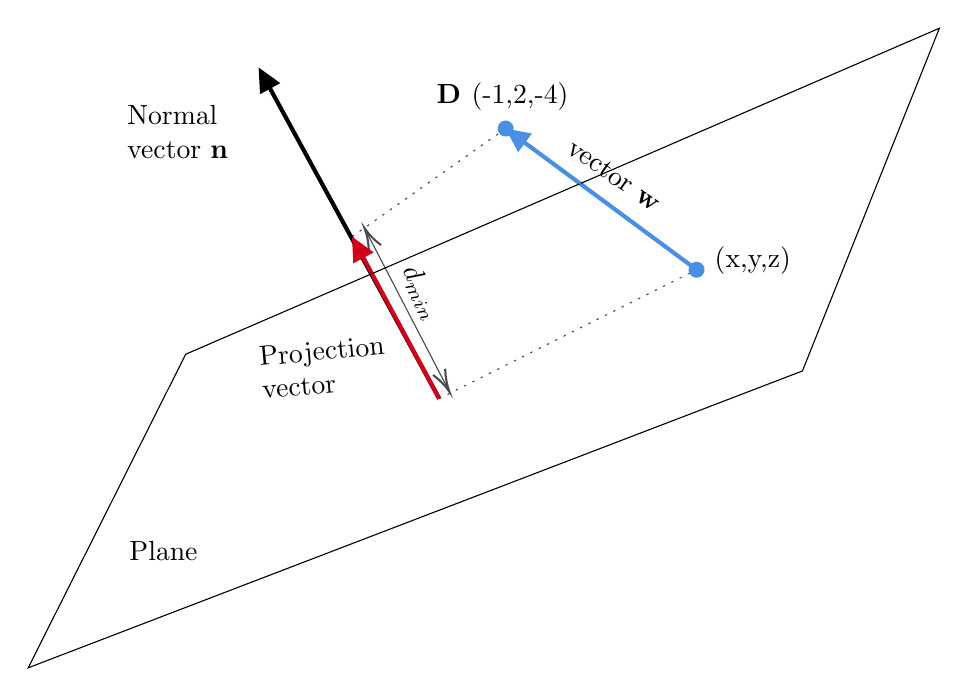
\begin{tikzpicture}[x=0.75pt,y=0.75pt,yscale=-1,xscale=1]
%uncomment if require: \path (0,324); %set diagram left start at 0, and has height of 324

%Straight Lines [id:da012474511036709712] 
\draw [color={rgb, 255:red, 74; green, 74; blue, 74 }  ,draw opacity=1 ] [dash pattern={on 0.84pt off 2.51pt}]  (165.51,108.36) -- (239.51,56.27) ;
%Straight Lines [id:da164610693713777] 
\draw [color={rgb, 255:red, 74; green, 74; blue, 74 }  ,draw opacity=1 ] [dash pattern={on 0.84pt off 2.51pt}]  (207.51,186.36) -- (331.51,124.27) ;
%Straight Lines [id:da0009900971082483778] 
\draw [color={rgb, 255:red, 74; green, 74; blue, 74 }  ,draw opacity=1 ]   (211.58,181.43) -- (172.42,105.98) ;
\draw [shift={(171.5,104.2)}, rotate = 422.57] [color={rgb, 255:red, 74; green, 74; blue, 74 }  ,draw opacity=1 ][line width=0.75]    (10.93,-3.29) .. controls (6.95,-1.4) and (3.31,-0.3) .. (0,0) .. controls (3.31,0.3) and (6.95,1.4) .. (10.93,3.29)   ;
\draw [shift={(212.5,183.2)}, rotate = 242.57] [color={rgb, 255:red, 74; green, 74; blue, 74 }  ,draw opacity=1 ][line width=0.75]    (10.93,-3.29) .. controls (6.95,-1.4) and (3.31,-0.3) .. (0,0) .. controls (3.31,0.3) and (6.95,1.4) .. (10.93,3.29)   ;
%Straight Lines [id:da6317108471264852] 
\draw [line width=1.5]    (207.51,186.36) -- (122.42,30.38) ;
\draw [shift={(120.51,26.87)}, rotate = 421.39] [fill={rgb, 255:red, 0; green, 0; blue, 0 }  ][line width=0.08]  [draw opacity=0] (11.61,-5.58) -- (0,0) -- (11.61,5.58) -- cycle    ;
%Straight Lines [id:da4711513779445873] 
\draw [color={rgb, 255:red, 74; green, 144; blue, 226 }  ,draw opacity=1 ][line width=1.5]    (331.51,124.27) -- (242.72,58.64) ;
\draw [shift={(239.51,56.27)}, rotate = 396.47] [fill={rgb, 255:red, 74; green, 144; blue, 226 }  ,fill opacity=1 ][line width=0.08]  [draw opacity=0] (11.61,-5.58) -- (0,0) -- (11.61,5.58) -- cycle    ;
%Straight Lines [id:da281513313013386] 
\draw [color={rgb, 255:red, 208; green, 2; blue, 27 }  ,draw opacity=1 ][line width=1.5]    (207.51,186.36) -- (167.4,111.89) ;
\draw [shift={(165.51,108.36)}, rotate = 421.7] [fill={rgb, 255:red, 208; green, 2; blue, 27 }  ,fill opacity=1 ][line width=0.08]  [draw opacity=0] (11.61,-5.58) -- (0,0) -- (11.61,5.58) -- cycle    ;
%Shape: Polygon [id:ds23253650680866844] 
\draw   (85.38,164.99) -- (448.5,7.93) -- (382.5,173.07) -- (9.5,316.07) -- (9.5,316.07) -- cycle ;
%Straight Lines [id:da02842289374539675] 
\draw [color={rgb, 255:red, 74; green, 144; blue, 226 }  ,draw opacity=1 ]   (239.51,56.27) -- (331.51,124.27) ;
\draw [shift={(331.51,124.27)}, rotate = 36.47] [color={rgb, 255:red, 74; green, 144; blue, 226 }  ,draw opacity=1 ][fill={rgb, 255:red, 74; green, 144; blue, 226 }  ,fill opacity=1 ][line width=0.75]      (0, 0) circle [x radius= 3.35, y radius= 3.35]   ;
\draw [shift={(239.51,56.27)}, rotate = 36.47] [color={rgb, 255:red, 74; green, 144; blue, 226 }  ,draw opacity=1 ][fill={rgb, 255:red, 74; green, 144; blue, 226 }  ,fill opacity=1 ][line width=0.75]      (0, 0) circle [x radius= 3.35, y radius= 3.35]   ;

% Text Node
\draw (56,44) node [anchor=north west][inner sep=0.75pt]   [align=left] {Normal \\vector \textbf{n} };
% Text Node
\draw (118.97,160.37) node [anchor=north west][inner sep=0.75pt]  [rotate=-354.79] [align=left] {Projection \\vector};
% Text Node
\draw (205,33) node [anchor=north west][inner sep=0.75pt]   [align=left] {\textbf{D }(-1,2,-4)};
% Text Node
\draw (339,112) node [anchor=north west][inner sep=0.75pt]   [align=left] {(x,y,z)};
% Text Node
\draw (272.66,59.12) node [anchor=north west][inner sep=0.75pt]  [rotate=-34.52] [align=left] {vector \textbf{w} };
% Text Node
\draw (198.69,119.24) node [anchor=north west][inner sep=0.75pt]  [rotate=-64.65] [align=left] {$d_{min}$};
% Text Node
\draw (57,254.07) node [anchor=north west][inner sep=0.75pt]   [align=left] {Plane};


\end{tikzpicture}
}
\caption{Triangle ABC and DBC}
\label{eq:solutions/1/27/myfig}
\end{figure}
In $\triangle{ABC}$, $\vec{M}$ is midpoint of hypotenuse AB, thus 
\begin{align}
&\vec{M} = \frac{\vec{A}+\vec{B}}{2}\label{eq:solutions/1/27/eq1} \\
&2\vec{M} = \brak{\vec{A+B}}\\
&\brak{\vec{A-M}} = \brak{\vec{M-B}}\\
&\norm{\vec{A}-\vec{M}}=\norm{\vec{M}-\vec{B}}\label{eq:solutions/1/27/eq4} \\
&\vec{M} = \frac{\vec{C}+\vec{D}}{2}\label{eq:solutions/1/27/eq2} \\
&2\vec{M} = \brak{\vec{C+D}}\\
&\brak{\vec{C-M}} = \brak{\vec{M-D}}\\
&\norm{\vec{C}-\vec{M}}=\norm{\vec{M}-\vec{D}}\label{eq:solutions/1/27/eq5} \\
&\vec{M} = \frac{\vec{A}+\vec{B}}{2} = \frac{\vec{C}+\vec{D}}{2}\label{eq:solutions/1/27/eq3} \\
&\vec{A - C} = \vec{A - M} + \vec{M - C} \\
&\vec{A - C} = \vec{M - B} + \vec{D - M} \\
&(\vec{A - C}) = k(\vec{D - B})\label{eq:solutions/1/27/eq6} \quad\text{[k value is 1]}
\end{align} 
Now from equation \eqref{eq:solutions/1/27/eq6} we can say that 
\begin{align}
&AC \parallel DB\label{eq:solutions/1/27/eq8} \\
&\norm{\vec{A - C}} = \norm{\vec{D - B}}\label{eq:solutions/1/27/eq7} 
\end{align}
Now it is given that AC $\perp$ BC, using this we can prove that DB $\perp$ BC. 
\begin{align}
&(\vec A -\vec C)^T(\vec{B}-\vec{C}) = 0 \\
&(\vec A -\vec M +\vec M -\vec C)^T(\vec{B}-\vec{C}) = 0 \\
&(\vec M -\vec B +\vec D -\vec M)^T(\vec{B}-\vec{C}) = 0 \\
&(\vec D -\vec B)^T(\vec{B}-\vec{C}) = 0 \\
&\implies DB \perp BC \\
&\vec{A - B} = \vec{A - C}+\vec{C - B} \\
&\vec{A - B} = \vec{B - D}+\vec{C - B} \quad\text{[From \eqref{eq:solutions/1/27/eq7}]} \\
&\vec{A - B} = \vec{C - D} \\
&\vec{A - B} = \vec{C - M}+ \vec{M - D} \\
&\vec{A - B} = \vec{C - M}+\vec{C - M} \quad\text{[From \eqref{eq:solutions/1/27/eq5}]}
\end{align} 
\begin{align}
&\vec{A - B} = 2 (\vec{C - M}) \\
&\vec{C - M} = \frac{1}{2}(\vec{A - B}) \\
&\norm{\vec{C - M}} = \frac{1}{2}\norm{\vec{A - B}}\label{eq:solutions/1/27/eqFin1}
\end{align}
Hence from \eqref{eq:solutions/1/27/eqFin1} proved,\\CM = $\frac{1}{2}$ AB
